\documentclass[12pt]{article}
%--------------------   start of the 'preamble'
%
\usepackage{graphicx,amssymb,amstext,amsmath,color}
\usepackage[margin=2cm]{geometry}
\usepackage{abstract}
\usepackage{setspace}
\usepackage[footnotesize,bf]{caption}

% TABLE
\usepackage{multicol,hhline,colortbl,multirow}
\usepackage{braket}
\usepackage{siunitx}
\usepackage{hyperref}
\usepackage{authblk}
\usepackage{siunitx}
\usepackage{mathrsfs}
%%\usepackage[sort&compress]{natbib}
%%\bibpunct{(}{)}{,}{a}{, }{;}
%
\usepackage[sort&compress]{natbib}
\bibpunct{[}{]}{,}{s}{}{;}


\definecolor{gray}{gray}{0.8}
\def\mobunits{\square\centi\meter\per\volt\per\second}
\def\gcm{\gram\per\cubic\centi\meter}
\def\ccg{\cellcolor{gray}}

\renewcommand{\labelitemii}{$\circ$}
\renewcommand{\bibname}{References}


\title{MorphCT Results - P3HT}
\author{Matthew Jones}
\date{\today}

\begin{document}
\maketitle

\section{Original Published Results}

\begin{center}
\begin{tabular}{| c | c | c | c | c | c | c |}
\hline
\rule{0pt}{2.5ex} 
\multirow{2}{*}{\textbf{ID}}&\multirow{2}{*}{\textbf{Simulation Name}}&\textbf{Density}&\textbf{Anisotropy}&\textbf{Anisotropy}&\textbf{Mobility}&\textbf{Intra-}\\
                            &&(\SI{}{\gcm})&(Arb. U.)&(Shape)&(\SI{}{\mobunits})&\textbf{\%}\\
\hhline{|=======|}
\textbf{\ccg1}&\rule{0pt}{2.5ex}\ccg p1-L15-f0.0-P0.1-T1.5-e0.5&\ccg 1.676&\ccg 0.2521&\ccg Disk&\ccg5.99$\times 10^{0}$&\ccg12\%\\
\textbf{2}&\rule{0pt}{2.5ex}p1-L15-f0.0-P0.1-T1.75-e0.5&1.061&0.0020&Spherical&6.24$\times 10^{-3}$&43\%\\
\textbf{\ccg3}&\rule{0pt}{2.5ex}\ccg p1-L15-f0.0-P0.1-T2.0-e0.5&\ccg 0.892&\ccg 0.0104&\ccg Spherical&\ccg5.16$\times 10^{-3}$&\ccg60\%\\
\textbf{4}&\rule{0pt}{2.5ex}p1-L15-f0.0-P0.1-T2.25-e0.5&0.787&0.0014&Spherical&4.80$\times 10^{-3}$&69\%\\
\textbf{\ccg5}&\rule{0pt}{2.5ex}\ccg p1-L15-f0.0-P0.1-T2.5-e0.5&\ccg 0.685&\ccg 0.0055&\ccg Spherical&\ccg4.71$\times 10^{-3}$&\ccg76\%\\
\hhline{-------}
\end{tabular}\label{table:mob}
\captionof{table}{The published results from MorphCT for the mobilities of pristine P3HT morphologies with varying disorder.
All simulations were performed using the NPT ensemble, which means that the densities vary significantly with temperature.}
\end{center}

\begin{figure}[h!]\centering
	\includegraphics[width=0.5\textwidth]{Figures/PublishedHoleMob.pdf}
    \caption{The mobility trend observed as a function of increasing temperature}
	\label{fig:MSD}
\end{figure}

Representative Values From Literature:
\begin{itemize}
    \item{Density: \SI{1.10}{\gcm}\cite{Newbloom2012a}}
\item{Mobility: \SI{1E-5}{} - \SI{1E-3}{\mobunits}\cite{Ballantyne2008b,Mauer2010,Pandey2000,Kim2006}}
\end{itemize}

Comments:
\begin{itemize}
    \item{Ordered mobility from system \textbf{1} significantly higher than literature, but disordered systems in excellent agreement.}
    \item{\textbf{1} exhibits significantly anisotropic charge transport, whereas \textbf{2}-\textbf{5} have approximately spherical carrier end-point distributions.}
    \item{There is a direct relationship between the density, mobility and intra-chain hopping percentage, however the effect of the density is unknown as it varies by 35\% between systems \textbf{2}-\textbf{5}, while reporting similar mobilities.
            Conversely, the 35\% decrease in the density of \textbf{1} and \textbf{2} results in a 3 order-of-magnitude decrease in mobility, and significant increase in the proportion of intra-chain hops in the system.}
\end{itemize}

\subsection{3D Carrier Network}

\begin{figure}[h!]\centering
	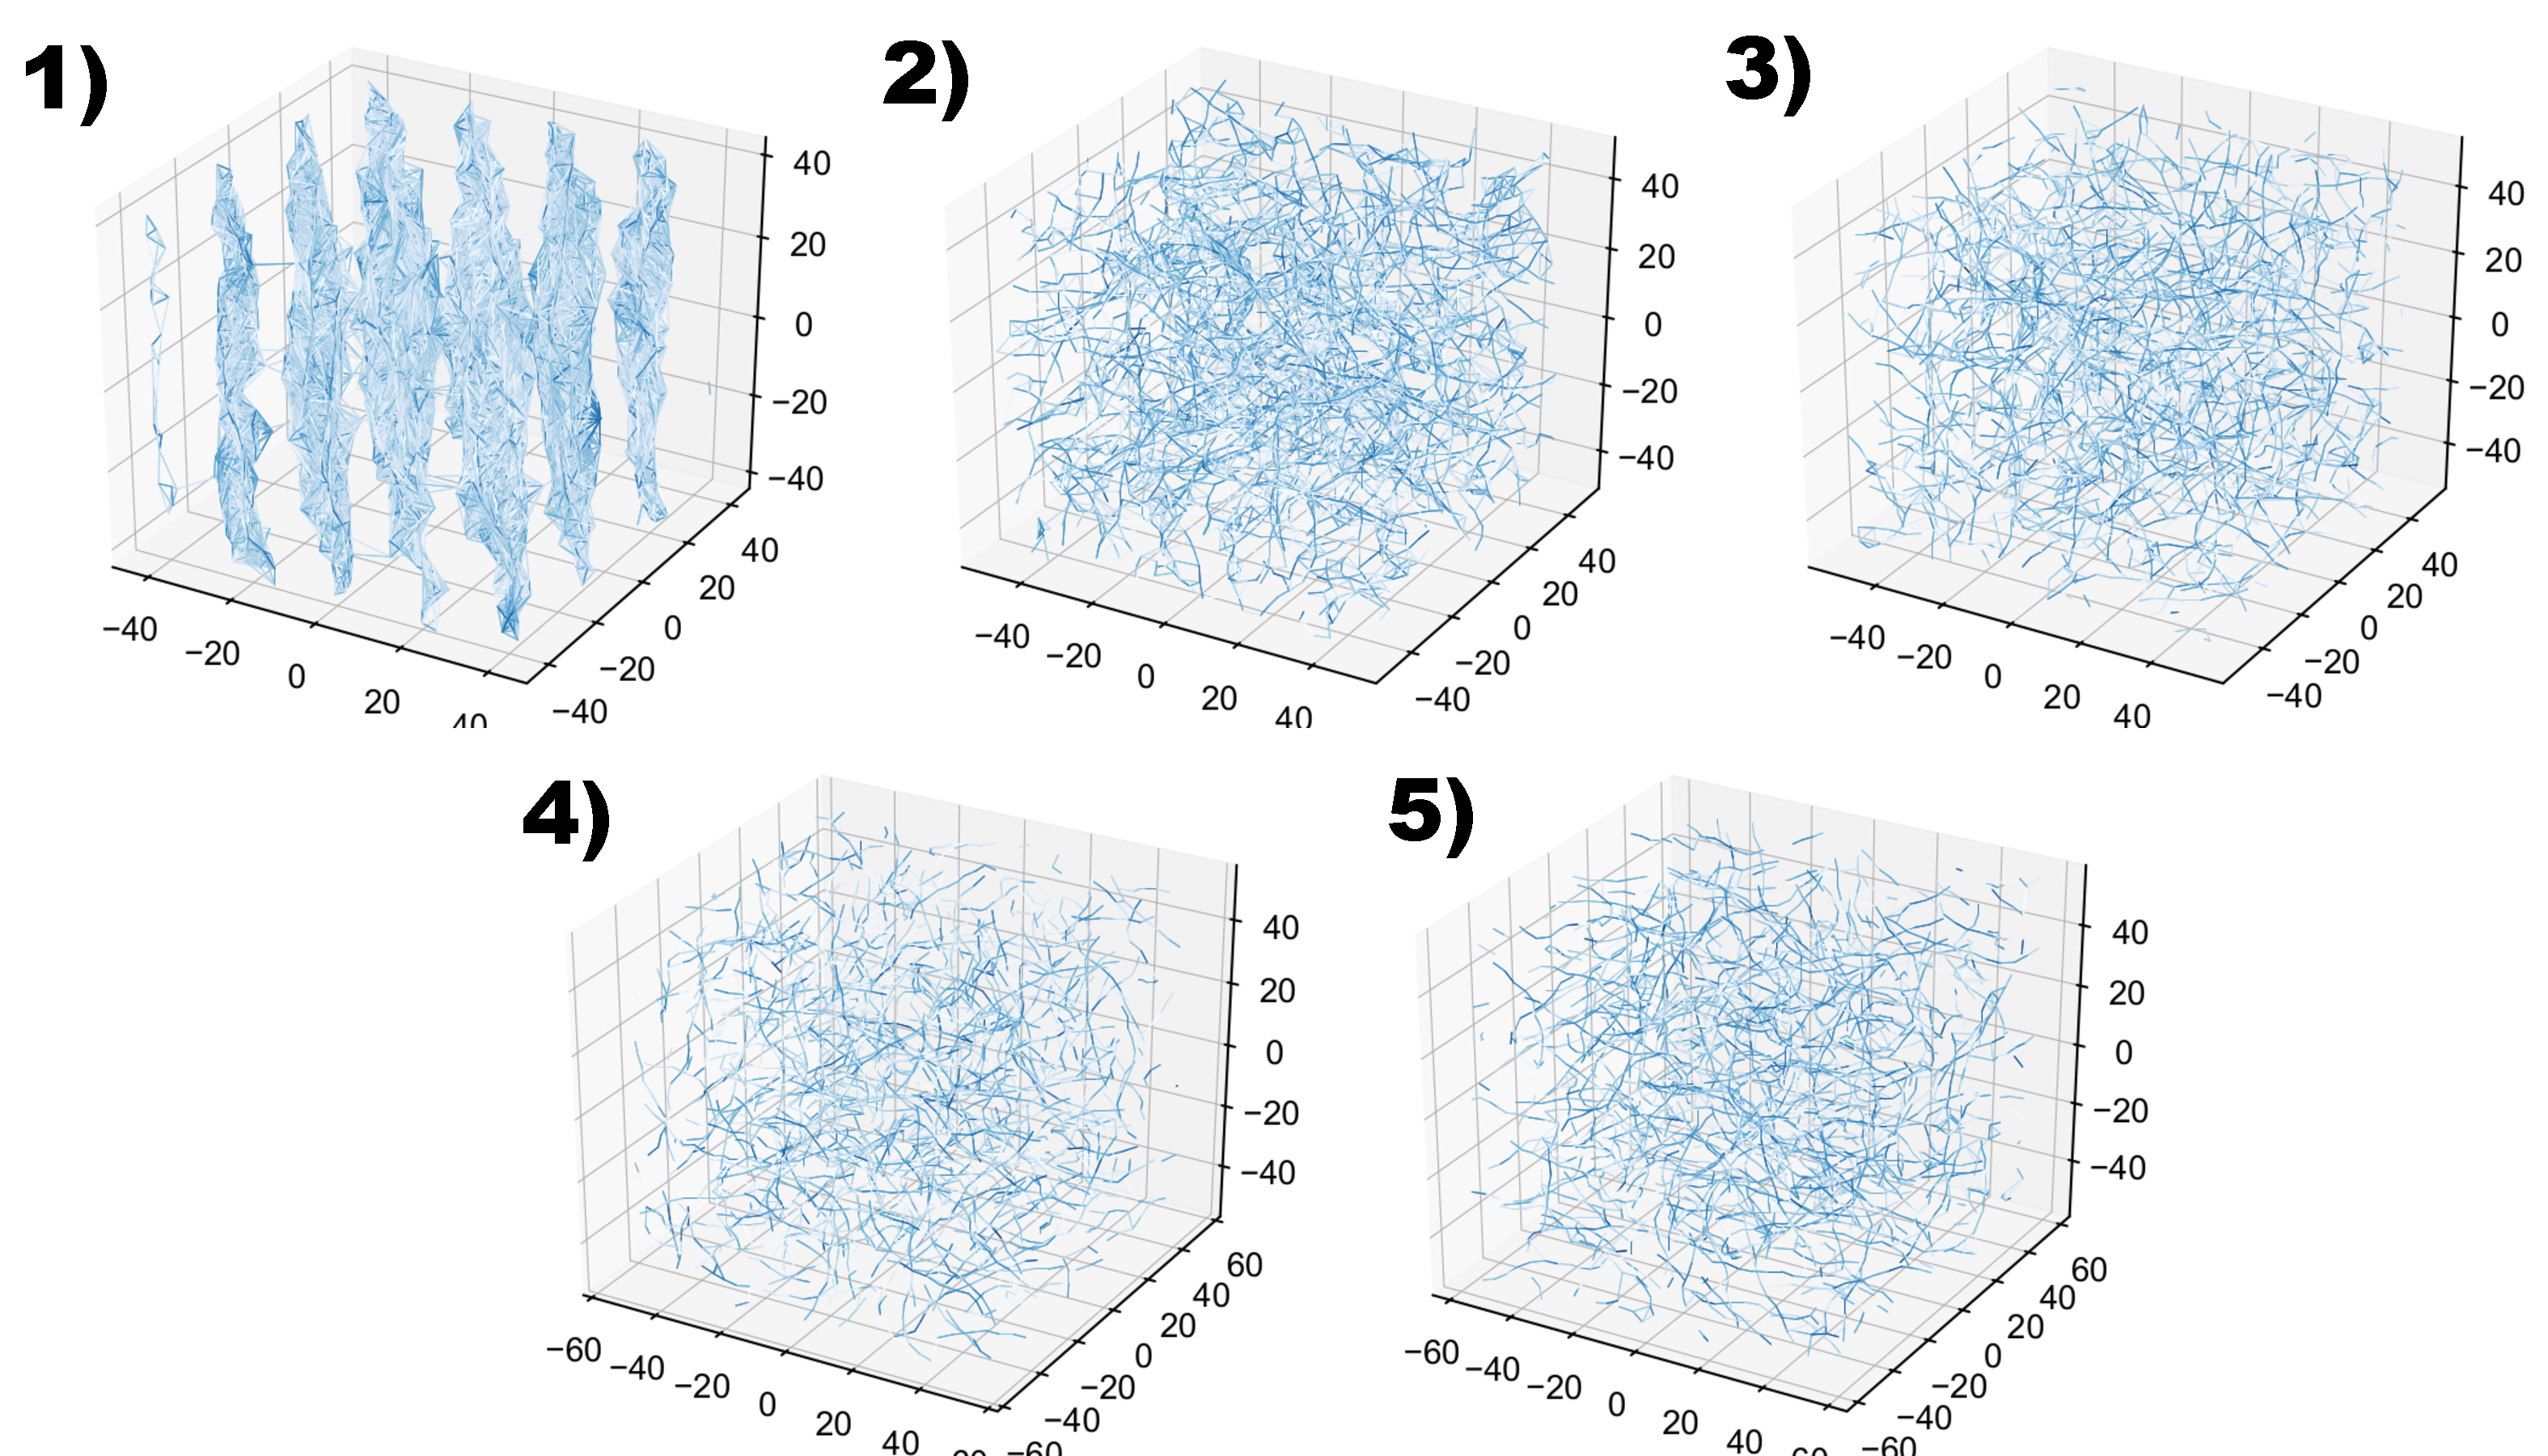
\includegraphics[width=\textwidth]{Figures/3dHole.pdf}
    \caption{The 3D heatmap of charge transport routes within the morphologies \textbf{1} - \textbf{5}.
    Dark routes describe commonly accessed hops between pairs of chromophores, whereas pale routes are less widely used in the KMC simulations.
    Each node therefore represents the location of a single chromophore.
The intensity value for the route is currently taken to be \texttt{I $=$ np.log10(freq) $/$ np.log10(max\_freq)}.}
	\label{fig:3dNetwork}
\end{figure}

Nothing unusual to see here.

\begin{itemize}
    \item{\textbf{1} has extremely ordered, anisotropic connections within layers, with a very small number of routes connecting the layers. 
        This acounts for the high mobility and the highly anisotropic disk-shaped distribution of carrier endpoints, as carriers tend to stay within the same layer, covering large distances in a short period of time due to the large number of connections.}
    \item{There isn't much to pick between the four disordered morphologies \textbf{2}-\textbf{5}.
        The number of connections and ratio of strong:weak connections appears to decrease from \textbf{2}-\textbf{5} as temperature increases, but otherwise the routes that carriers take through the morphologies look approximately the same.
    This accounts for the spherical distribution of endpoints and low anisotropies in the disordered systems.}
\end{itemize}


\subsection{MSDs}


\begin{figure}[h!]\centering
	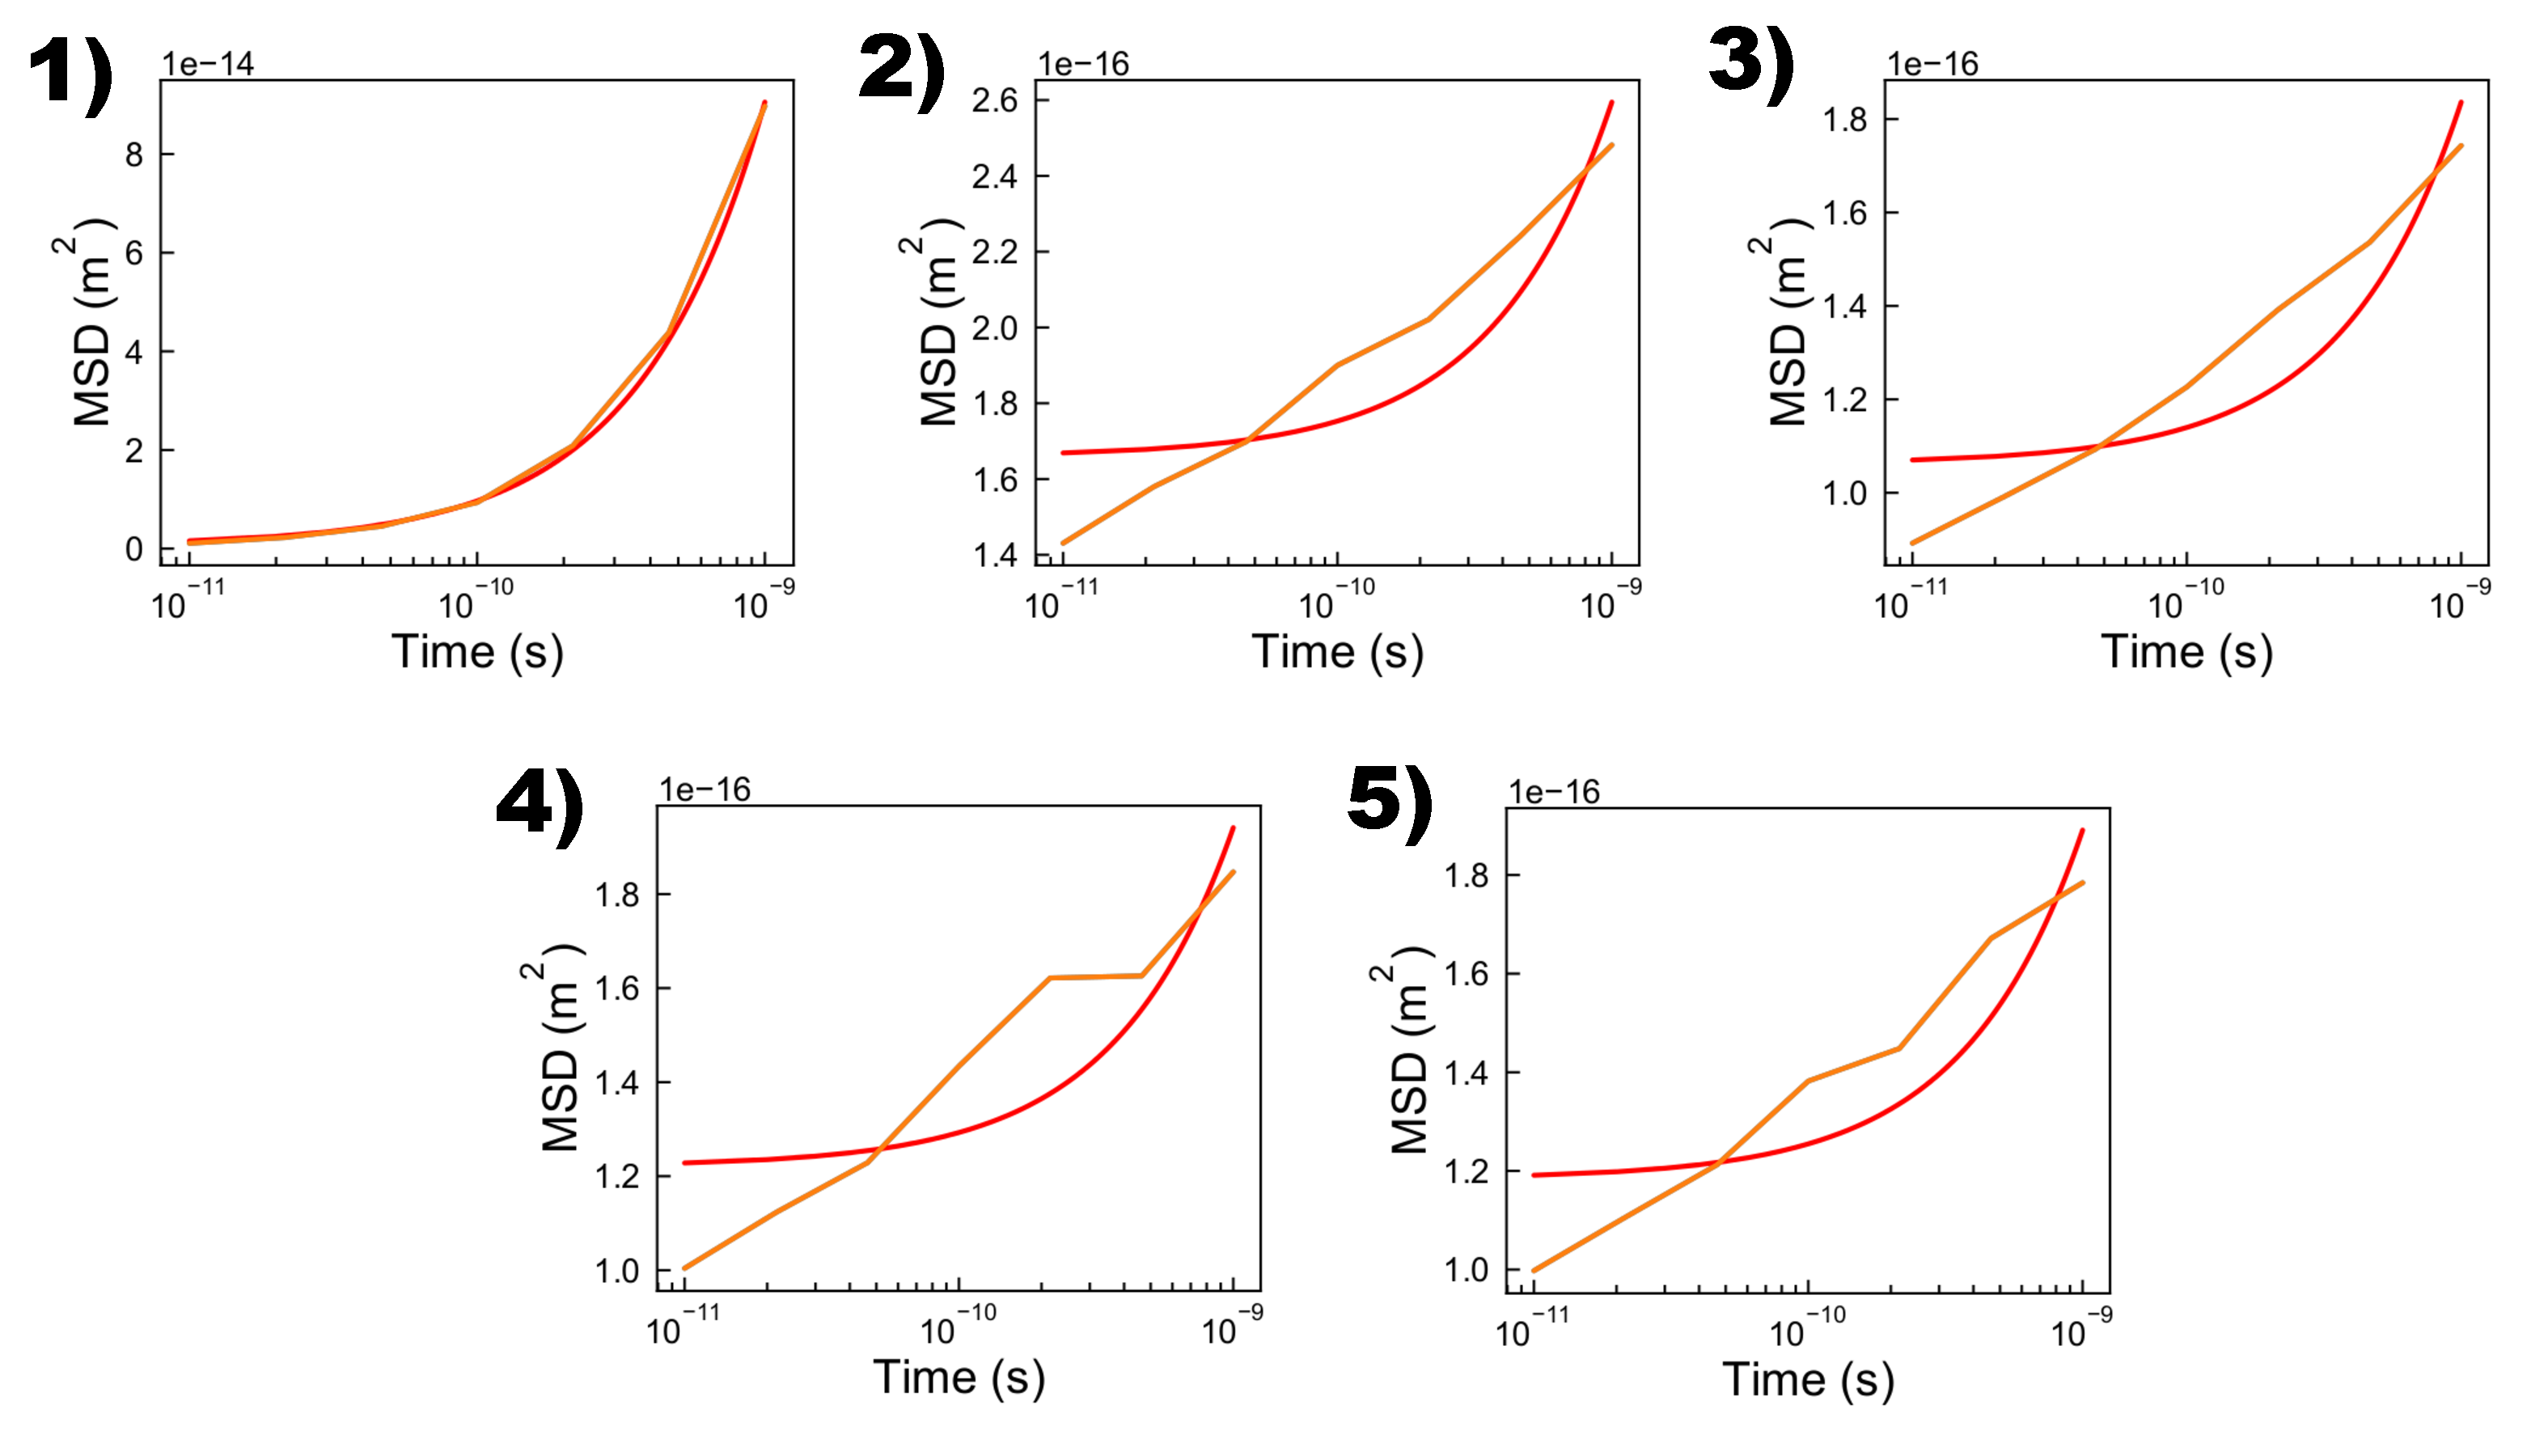
\includegraphics[width=\textwidth]{Figures/MSDHole.pdf}
    \caption{The semi-log-x mean squared displacement curves of the carriers within the morphologies \textbf{1} - \textbf{5}.}
	\label{fig:MSD}
\end{figure}


\begin{itemize}
    \item{The disordered fits are bloody awful, and this is due to the `saturation behaviour', i.e. the MSD appears to have either different transients or converges to a particular value (the only way to work out which is by running the KMC for longer, but we are already pushing the boundary of how long we can run this for - the morphology autocorrelation time is of the order 10 ns, so we would be omitting significant morphological fluctuations if we were to run the KMC for any longer).
            This behaviour arises from the extremely preferential bias for carriers to hop intra-chain rather than inter-chain, especially in the disordered morphologies.
        Carriers therefore prefer to hop up and down the chain rather than increasing their displacement, regardless of the KMC simulation time.}
    \item{Fitting values vary from 99.97\% for \textbf{1}, through 90.64\%, 91.15\%, and 84.83\% for \textbf{2}, \textbf{3}, and \textbf{4} respectively, and 88.17\% for \textbf{5} (linear MSD for high mobility, ordered system but off-linear for disordered morphs due to saturation).} 
\end{itemize}


\subsection{Hopping Rate Distributions}

\begin{figure}[h!]\centering
	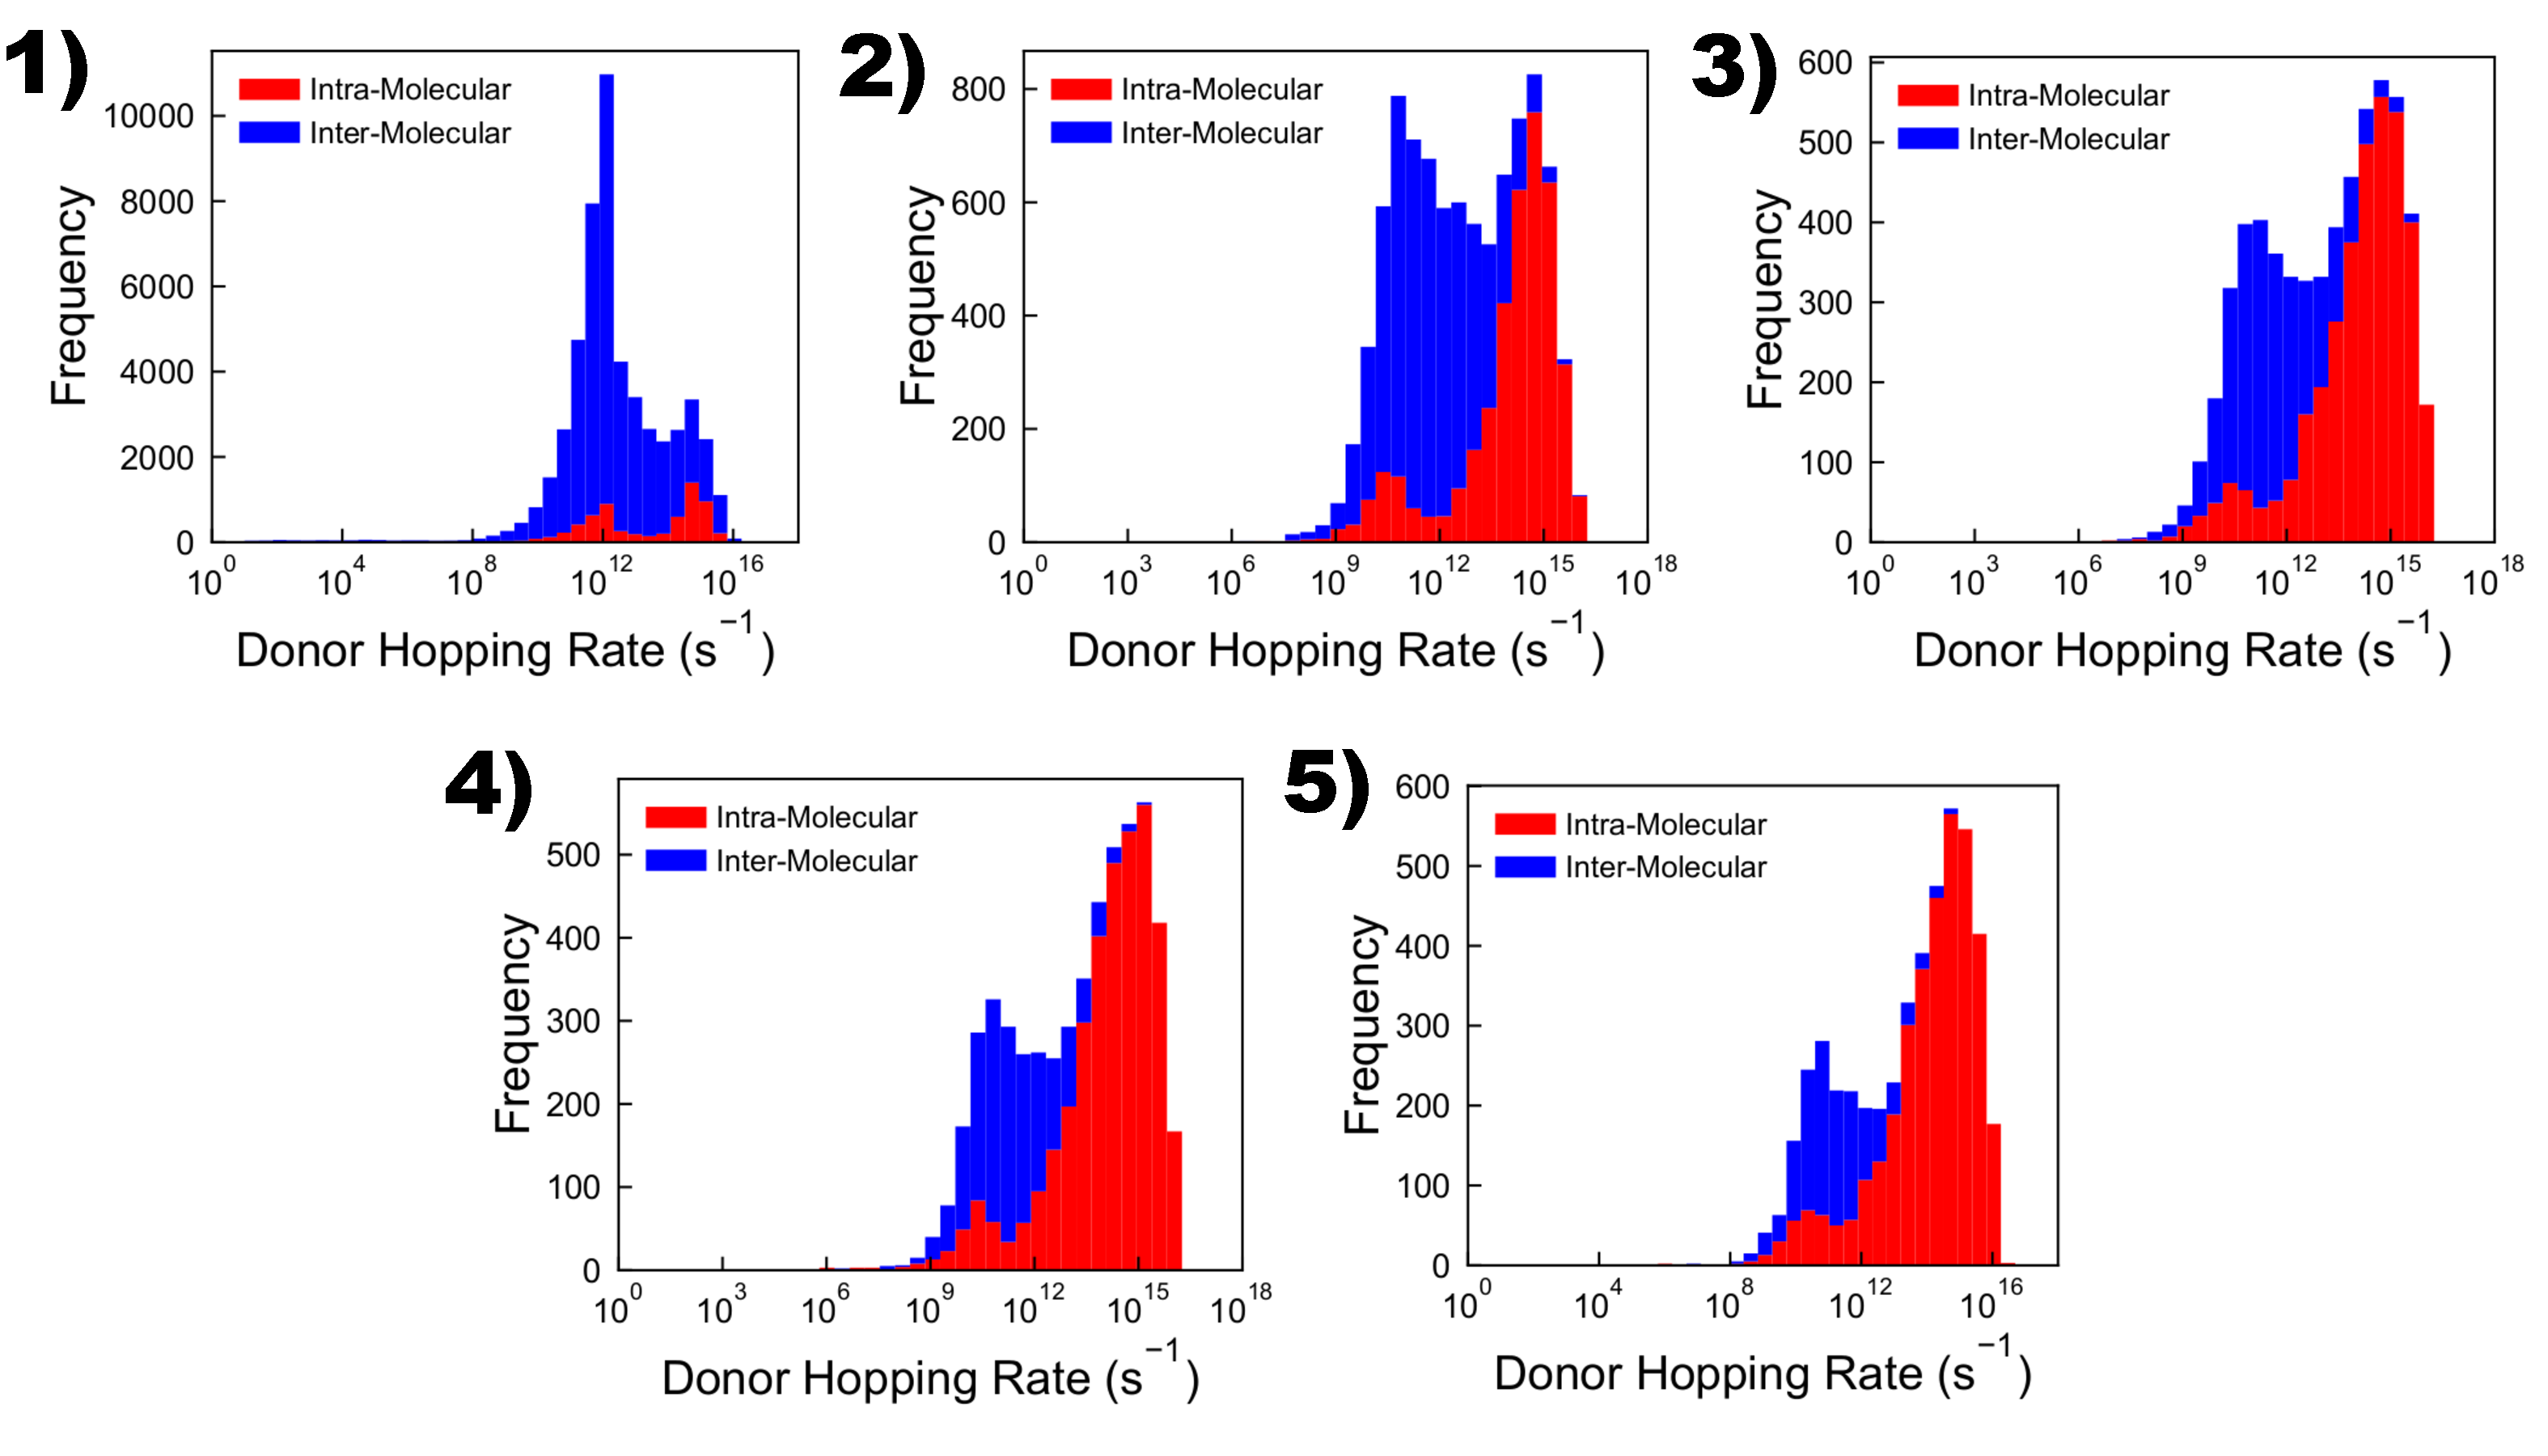
\includegraphics[width=\textwidth]{Figures/DonorHoppingRateMixed.pdf}
    \caption{The stacked hopping-rate distributions for intra- and inter-molecular hops executed by carriers within the morphologies \textbf{1} - \textbf{5}.}
	\label{fig:HoppingRateMixed}
\end{figure}

\clearpage

\begin{itemize}
    \item{The hopping rate distributions identify the reason for the difference in intra-chain hop proportion as a function of rate.}
    \item{The KMC algorithm queues up all possible hops and then executes the hop that has the shortest wait time.
        This naturally biases selection from the distribution to the higher hopping rates, as it is more likely that these rates will produce a shorter hopping time (although the value of the random number can affect this somewhat).
    In the disordered morphologies, the fastest hopping rates are almost completely dominated by intra-molecular hops along the chains, explaining why the intra-chain proportions for \textbf{2-5} in Table \ref{table:mob} are so much higher than in the ordered case \textbf{1}, where the proportion of hops that are intra- and inter-chain is more evenly split.}
    \item{The frequencies of hopping rates in \textbf{1} are significantly larger than in the disordered morphologies, due to the proximity of chromophores within the hopping limit (around 10 \AA) leading to a large number of possible connections for carriers to take.}
    \item{The bimodal peaks in all distributions most likely correspond to nearest- and next-nearest-neighbour hops. 
        A significant number of nearest-neighbour hops in the ordered morphology \textbf{1} are inter-molecular, resulting in larger distances covered in the same amount of time and therefore higher mobilities.
    In the disordered morphologies \textbf{2-5}, the nearest-neighbour peak is dominated by intra-molecular hops, and so charges become more likely to be trapped on the same chain, quenching inter-molecular motion and restricting mobility.}
\end{itemize}


\subsection{Scattering Data}
 
\begin{itemize}
    \item{I have skipped including the diffraction patterns as the ordered morphology showed a single, intense dot representing the long-range order of the lammelae, and the disordered morphologies had no discernable features.}
\end{itemize}

\clearpage

\section{Post-Shrink MorphCT Results}


\begin{center}
\begin{tabular}{| c | c | c | c | c | c | c |}
\hline
\rule{0pt}{2.5ex} 
\multirow{2}{*}{\textbf{ID}}&\multirow{2}{*}{\textbf{Simulation Name}}&\textbf{Density}&\textbf{Anisotropy}&\textbf{Anisotropy}&\textbf{Mobility}&\textbf{Intra-}\\
                            &&(\SI{}{\gcm})&(Arb. U.)&(Shape)&(\SI{}{\mobunits})&\textbf{\%}\\
\hhline{|=======|}
\textbf{\ccg6}&\rule{0pt}{2.5ex}\ccg sp1-L15-f0.0-P0.1-T1.5-e0.5&\ccg 1.676&\ccg 0.2521&\ccg Disk&\ccg5.99$\times 10^{0}$&\ccg12\%\\
\textbf{7}&\rule{0pt}{2.5ex}sp1-L15-f0.0-P0.1-T1.75-e0.5&1.676&0.0056&Spherical&4.73$\times 10^{-2}$&20\%\\
\textbf{\ccg8}&\rule{0pt}{2.5ex}\ccg sp1-L15-f0.0-P0.1-T2.0-e0.5&\ccg 1.676&\ccg 0.0008&\ccg Spherical&\ccg5.69$\times 10^{-3}$&\ccg20\%\\
\textbf{9}&\rule{0pt}{2.5ex}sp1-L15-f0.0-P0.1-T2.25-e0.5&1.676&0.0013&Spherical&1.97$\times 10^{-2}$&21\%\\
\textbf{\ccg10}&\rule{0pt}{2.5ex}\ccg sp1-L15-f0.0-P0.1-T2.5-e0.5&\ccg 1.676&\ccg 0.0007&\ccg Spherical&\ccg9.98$\times 10^{-3}$&\ccg21\%\\
\hhline{-------}
\end{tabular}\label{table:mob}
\captionof{table}{The results from MorphCT for the mobilities of the pristine P3HT morphologies with varying disorder.
All disordered simulations were shrunk down for 1E6 timesteps with a dt $= 0.001$, at which point the simulation box dimensions were the same as the ordered morphology, resulting in a density of \SI{1.676}{\gcm}.}
\end{center}

\begin{figure}[h!]\centering
	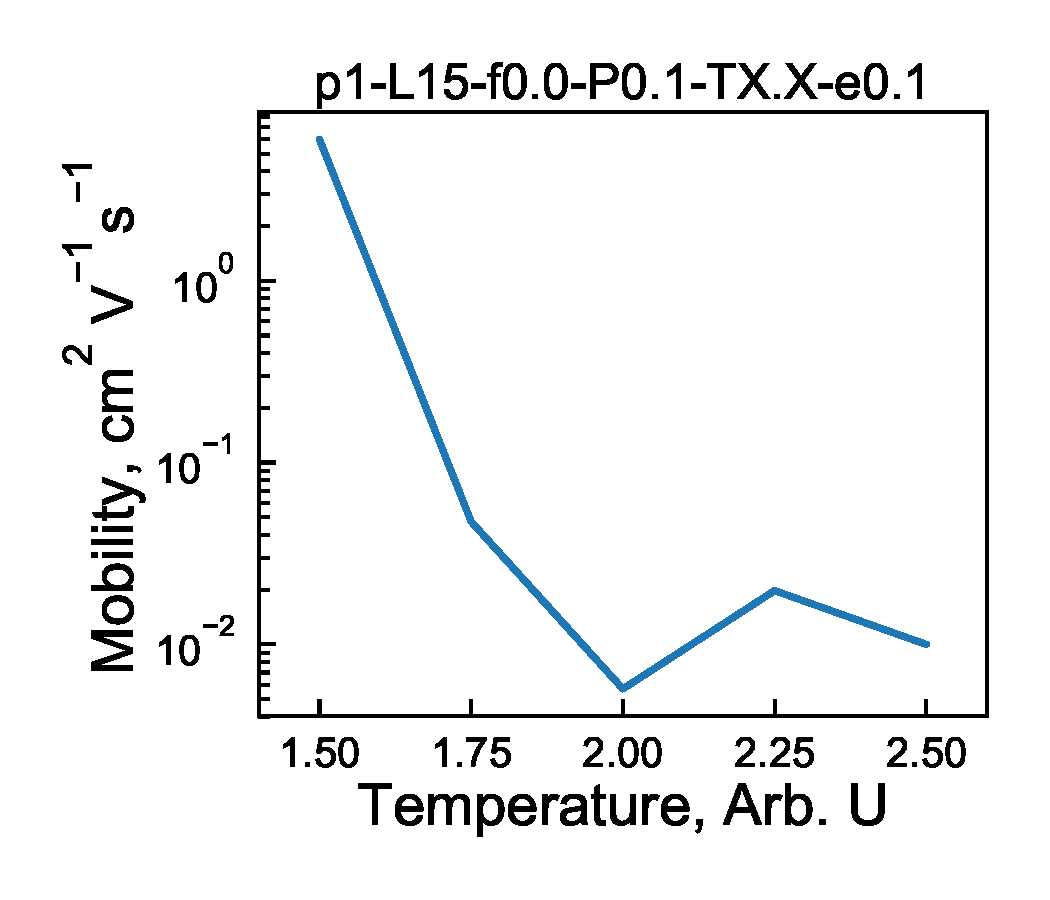
\includegraphics[width=0.5\textwidth]{Figures/ShrunkMobilityHole.pdf}
    \caption{The mobility trend of the shrunk morphologies, observed as a function of increasing temperature.
    It is expected that, now the densities are constant, the variation in mobility is a function of structural order alone.}
	\label{fig:MSD}
\end{figure}


\begin{itemize}
    \item{There is now more variation between the disordered morphologies than before, but the general trend is as it was.}
    \item{Additionally, the intra-chain hopping percentages have been reconciled somewhat with all morphologies exhibiting a similar percentage of intra-chain hops.}
\end{itemize}


\subsection{3D Carrier Network}

\begin{figure}[h!]\centering
	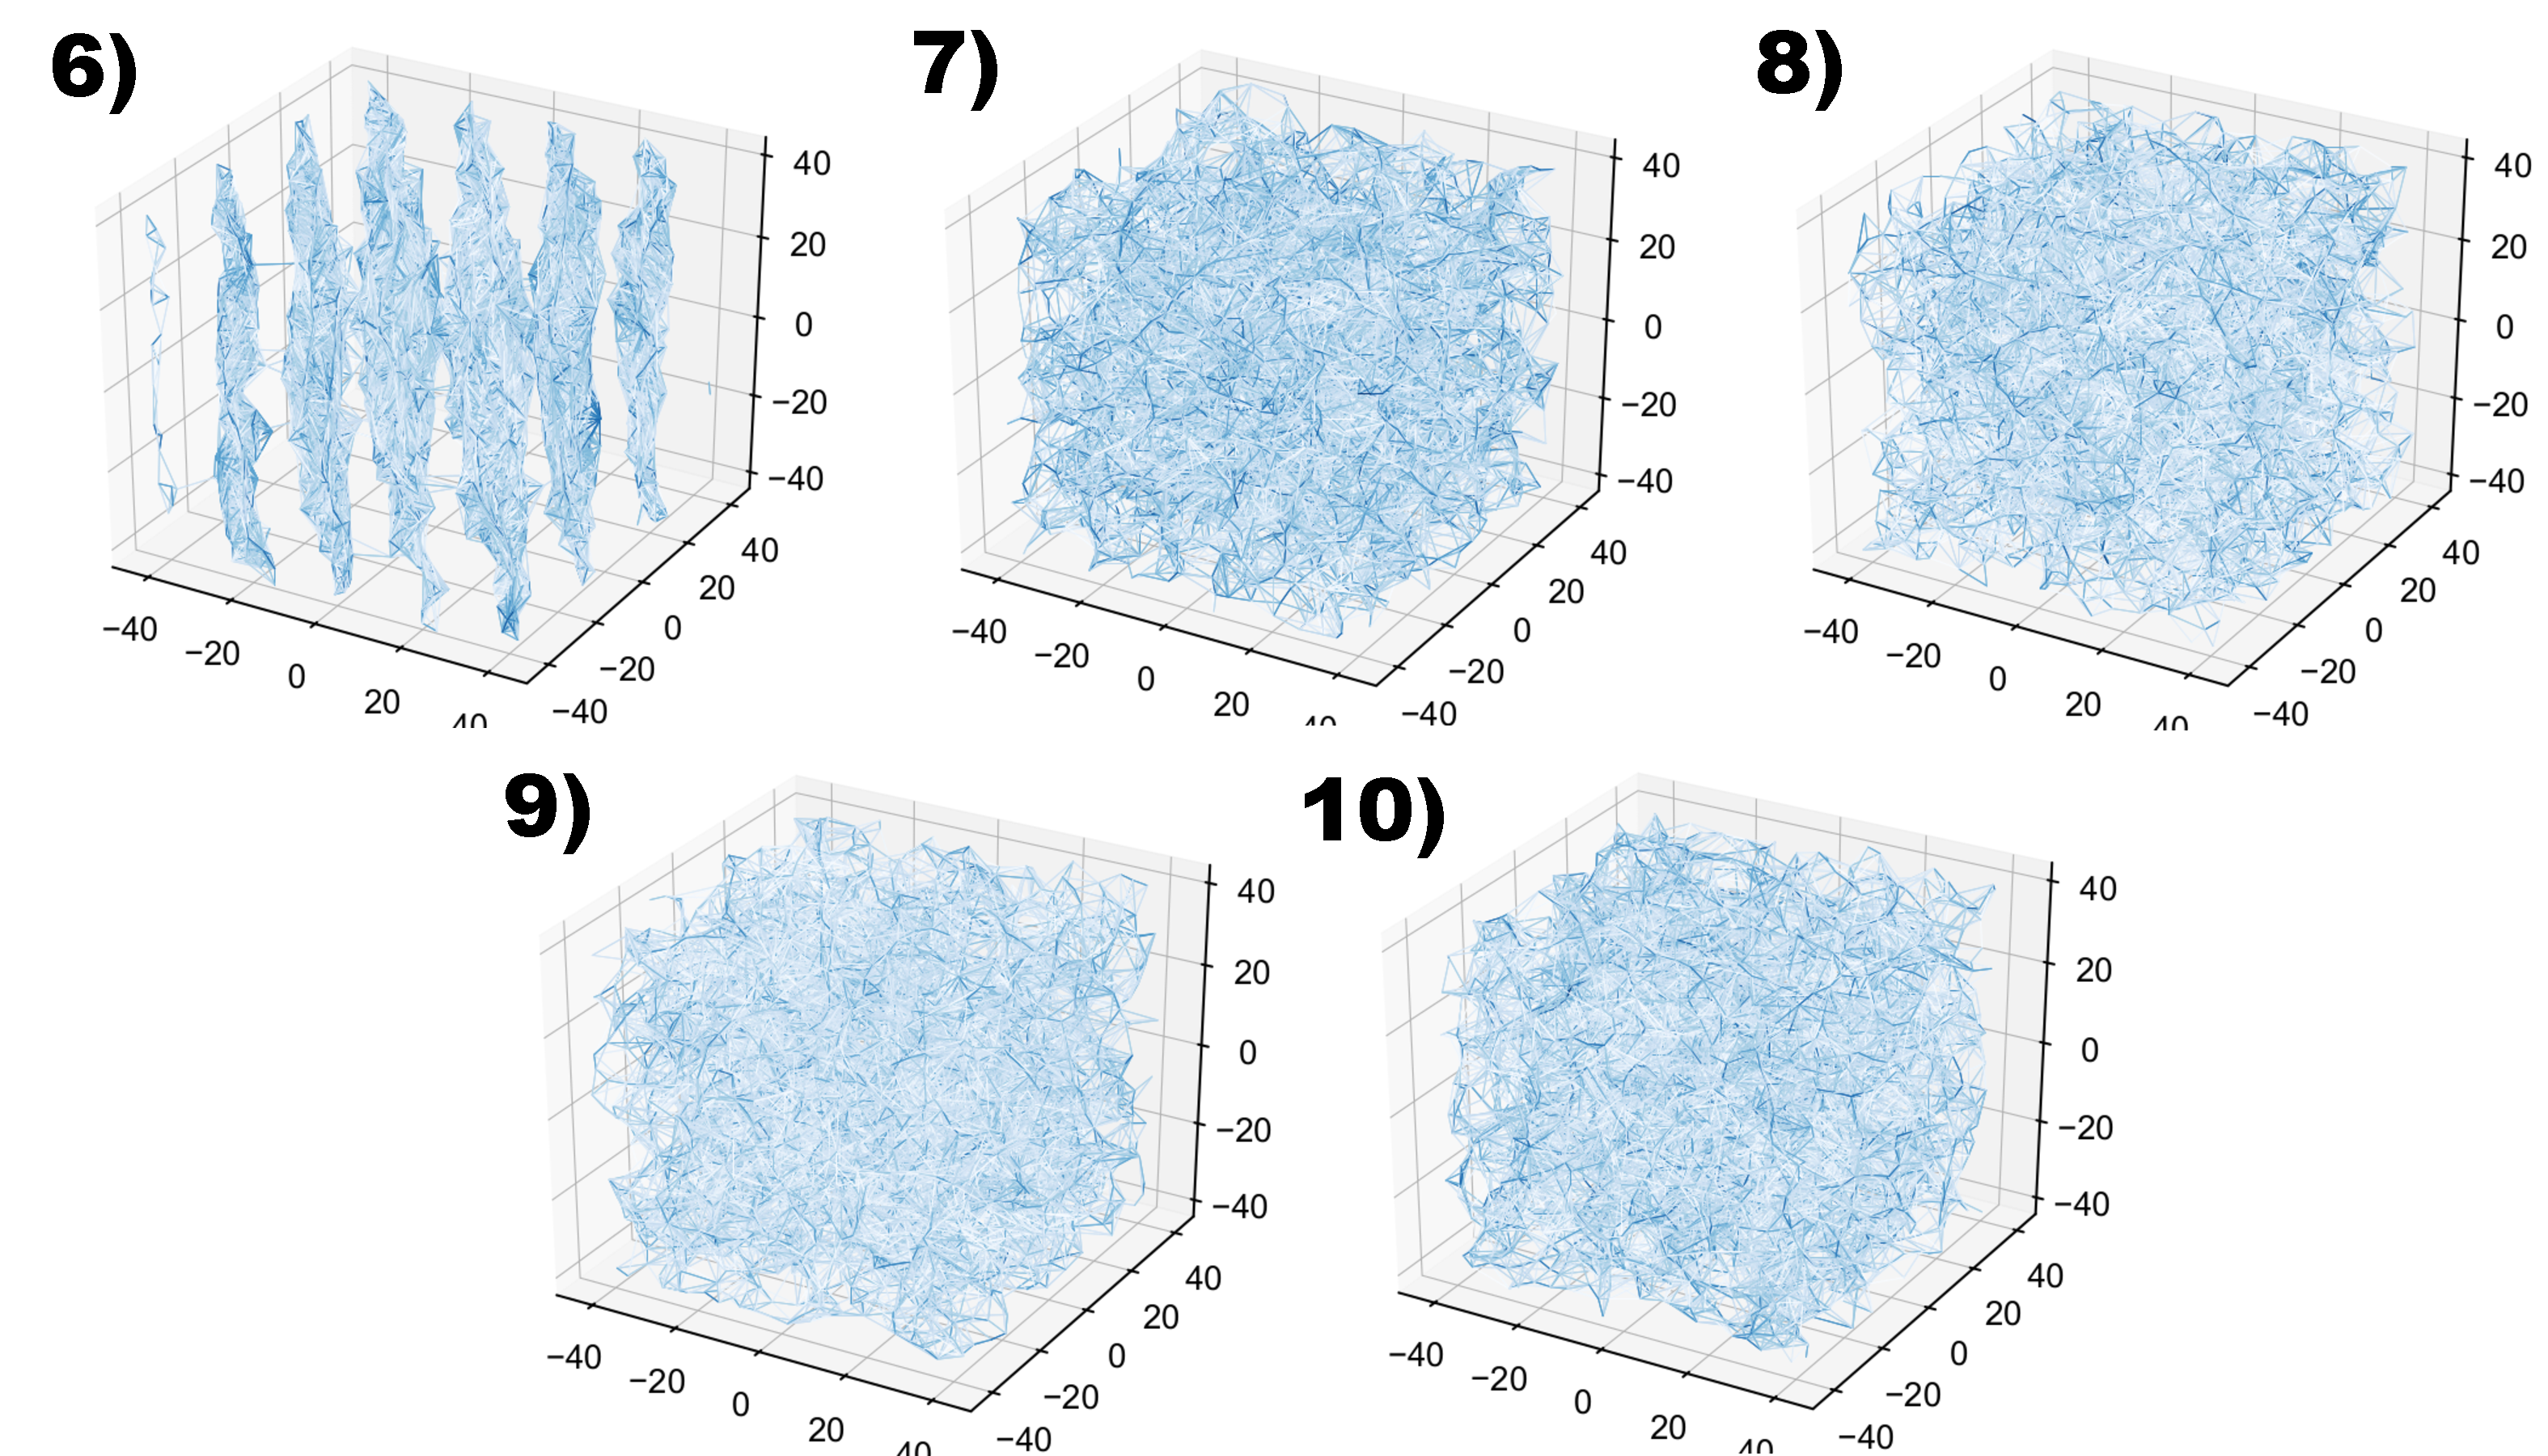
\includegraphics[width=\textwidth]{Figures/Shrunk3dHole.pdf}
    \caption{The 3D heatmap of charge transport routes within the morphologies \textbf{6} - \textbf{10}.
    Dark routes describe commonly accessed hops between pairs of chromophores, whereas pale routes are less widely used in the KMC simulations.
    Each node therefore represents the location of a single chromophore.
The intensity value for the route is currently taken to be \texttt{I $=$ np.log10(freq) $/$ np.log10(max\_freq)}.}
	\label{fig:3dNetwork}
\end{figure}

\begin{itemize}
    \item{Without some quantitative analysis, it's difficult to note any differences here, although \textbf{9} is noticably paler than the other disordered morphologies. 
        This indicates that there are fewer heavily-used, fast routes through the morphology.
    However, the mobility of \textbf{9} is not significantly lower, suggesting that either more frequently-used routes occur deeper within the morphology and are so not visible on these graphs, or that this analysis is not particularly well-suited to explaining the mobility trends.}
\end{itemize}


\subsection{MSDs}

\begin{figure}[h!]\centering
	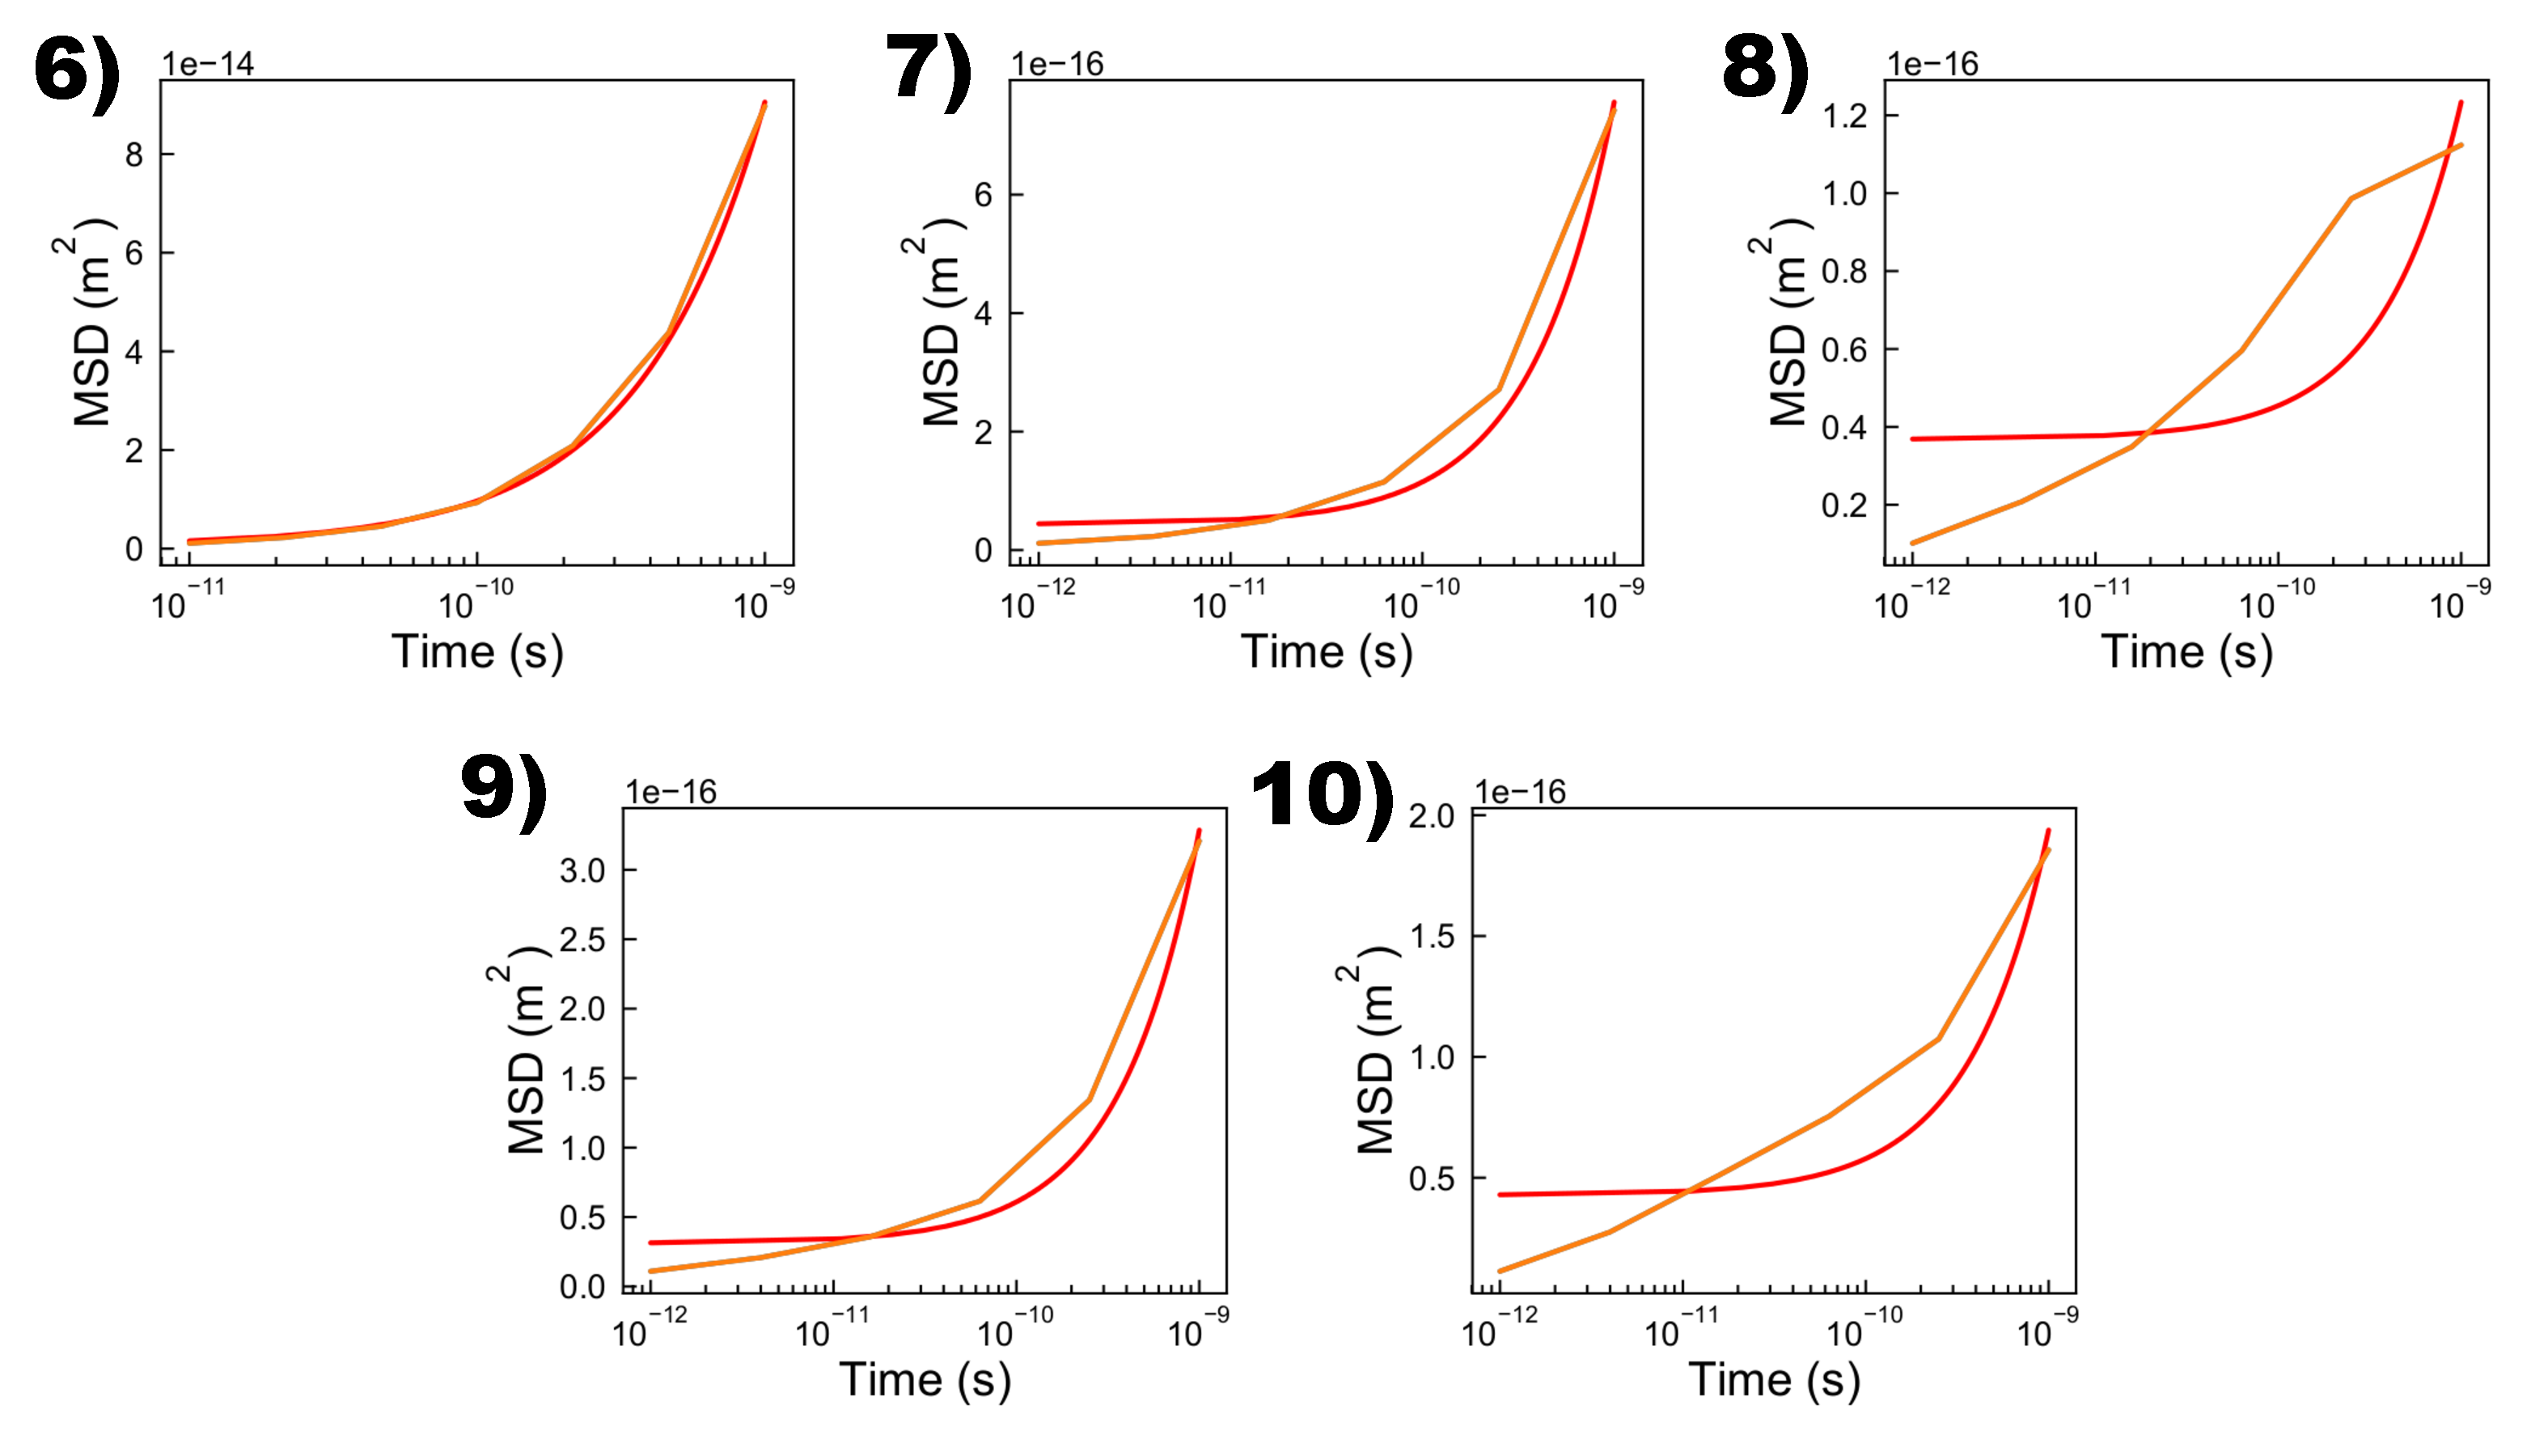
\includegraphics[width=\textwidth]{Figures/ShrunkMSDHole.pdf}
    \caption{The semi-log-x mean squared displacement curves of the carriers within the morphologies \textbf{6} - \textbf{10}.}
	\label{fig:MSD}
\end{figure}


\begin{itemize}
    \item{Simulations \textbf{8} and \textbf{10} are still pretty bad, but there has been a significant improvement in the linear trends observed in \textbf{7} and \textbf{9}, due to the minimization of the previous saturation behaviour.}
    \item{The fits for \textbf{8} and \textbf{10} look to be underestimating the mobility compared to the other two disordered morphologies \textbf{7} and \textbf{9}. I doubt it's a coincidence that the two simulations with the worst fits are the ones which have the lowest mobilities.}
\end{itemize}


\subsection{Hopping Rate Distributions}


\begin{figure}[h!]\centering
	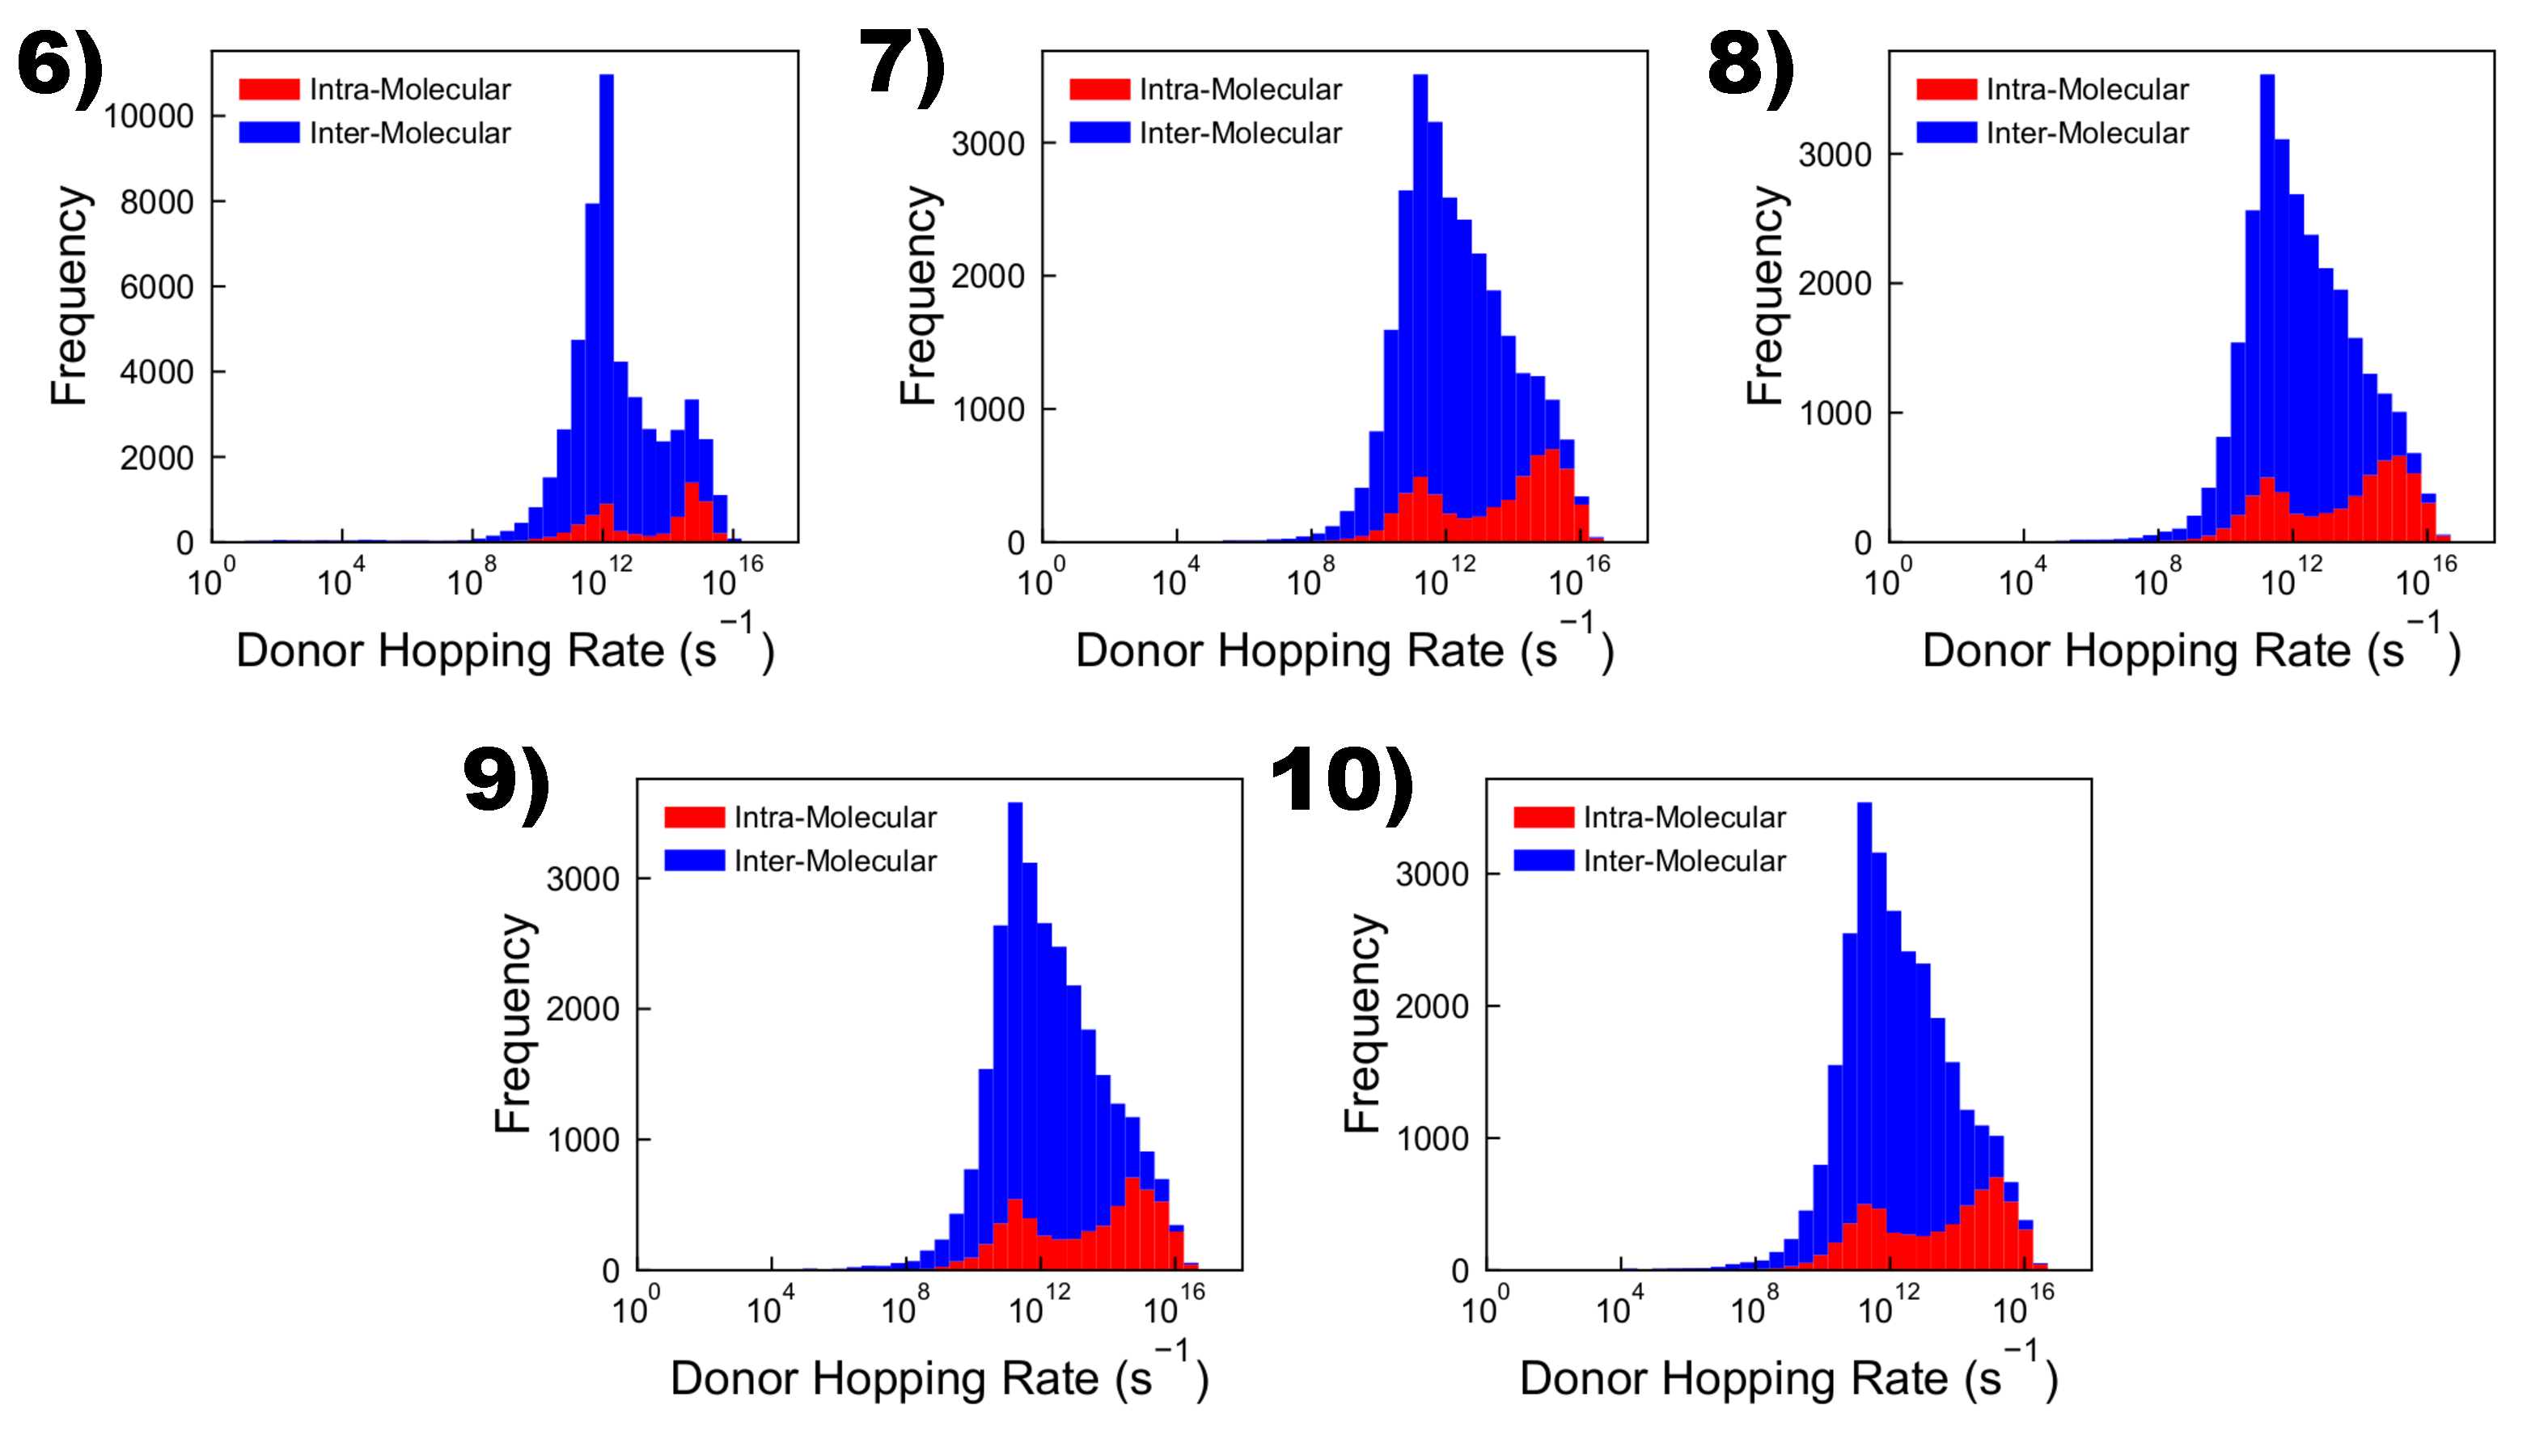
\includegraphics[width=\textwidth]{Figures/ShrunkDonorHoppingRateMixed.pdf}
    \caption{The stacked hopping-rate distributions for hops executed by carriers within the morphologies \textbf{1} - \textbf{5}.
    Note that currently MorphCT cannot distinguish inter- and intra-molecular hops when }
	\label{fig:HoppingRateMixed}
\end{figure}

\begin{itemize}
    \item{As before, the frequencies of each hopping rate are generally higher for the ordered morphology, \textbf{6}, than in the disordered systems, \textbf{7}-\textbf{10}.
        This is due to better packing resulting in a larger quantity of viable hopping targets, given a particular initial chromophore.}
    \item{The hopping rate frequencies are higher for the disordered morphologies \textbf{7}-\textbf{10} than they were for \textbf{2}-\textbf{5}.
        This makes sense - the density in \textbf{7}-\textbf{10} is significantly higher than in \textbf{2}-\textbf{5}, and so chromophores are closer together, resulting in a larger quantity of viable hopping targets.}
    \item{Unlike the simulations \textbf{1}-\textbf{5}, where the highest hopping rates were predominantly intra-molecular, the hopping rate distributions for \textbf{6}-\textbf{10} are more balanced between hops along- and between-the-chains.
        This is also reflected by the $\sim$ 20\% intra-chain hop percentage, which is significantly lower than for the low-density simulations.}
    \item{There is no discernable difference between the disordered simulations \textbf{7}-\textbf{10}. This would imply that the noisy (within 1 order of magnitude) mobility data could be the result of short KMC simulations, however longer simulations did not seem to affect the mobility values significantly.}
\end{itemize}

\clearpage

\section{Outstanding Questions}


\begin{itemize}
    \item{Why are the MSD fits so bad for \textbf{8} and \textbf{10}, even though their hopping rate distributions looks identical to the other disordered morphologies, and the ratio of intra- to inter-chain hops the same?}
    \item{Why does a bad MSD fit appear to correspond to a lower mobility in morphologies of the same density?}
    \item{How do we get about an order-of-magnitude variation in the mobility, even though the density and hopping-rate distributions look generally the same?}
\end{itemize}


\bibliography{refs}
\bibliographystyle{unsrt}


\end{document}
